\section{Introduction}
\label{sec:intro}

The study of neural scaling laws, which predictably map training resources to model performance, is a cornerstone of modern language modeling research and engineering.
% \bmg{I think citations after that would be nice, happy to add them just unsure if you'd be happy with edits...}
% \rylan{I think the rest of the introduction contains the citations.}
\citet{hestness2017deeplearningscalingpredictable} and soon after \citet{kaplan2020scaling} laid the foundation by demonstrating that pretraining losses scale as power laws with the number of data points, model parameters and pretraining compute. This was followed by significant additional work in the ensuing years (Sec.~\ref{sec:related_work} Related Work).
Such discoveries led to the modern paradigm of training extremely large language models \citep{openai2024gpt4technicalreport, gemini2025gemini2p5, deepseekai2025deepseekv3technicalreport, yang2025qwen3technicalreport,kimiteam2025kimik2openagentic,5team2025glm45agenticreasoningcoding}.


\begin{table*}[t]
\centering
\setlength{\tabcolsep}{3pt}
\footnotesize
\begin{tabular}{rrrrrr|r|rr}
\toprule
\multicolumn{7}{c|}{Table A9 from \citet{hoffman2022chinchilla}} & \multicolumn{2}{c}{Our Contribution} \\
\midrule
d\_model &  ffw\_size &  kv\_size &  n\_heads &  n\_layers & n\_vocab & \makecell{Chinchilla's\\Reported\\Model\\Parameters (M)} & \makecell{Best Fit\\Formula's\\Model\\ Parameters (M)} & \makecell{Standard\\Formula's\\Model\\Parameters (M)}\\
\midrule
    512 & 2048 & 64 & 8 & 8 & 32168 & 44 & 44 & 42 \\ 
    576 & 2304 & 64 & 9 & 9 & 32168 & 57 & 57 & 54 \\ 
    640 & 2560 & 64 & 10 & 10 & 32168 & 74 & 74 & 70 \\ 
    \vdots & \vdots & \vdots & \vdots & \vdots & \vdots & \vdots & \vdots & \vdots\\
    4864 & 19456 & 128 & 36 & 47 & 32168 & 13775 & 14319 & 13266 \\ 
    4992 & 19968 & 128 & 32 & 49 & 32168 & 14940 & 14939 & 13937 \\ 
    5120 & 20480 & 128 & 40 & 47 & 32168 & 16183 & 16182 & 14950 \\ 
\bottomrule
\end{tabular}
\caption{\textbf{Three Interpretations of Chinchilla's Model Parameters.}
\citet{hoffman2022chinchilla}'s Table A9 provides architectural hyperparameters of models used in the Chinchilla analyses, along with corresponding model parameters.
However, two alternative interpretations of model parameters are possible: model parameters calculated from architectural hyperparameters using a ``standard'' formula (Eqn.~\ref{eqn:standard}) and model parameters calculated from architectural hyperparameters using a ``best fit'' formula (Eqn.~\ref{eqn:bestfit}). Appendix~\ref{app:sec:chinchilla_table_a9}.
}
\label{tab:all_models_abridged}
\end{table*}


\begin{figure*}[t!]
    \centering
    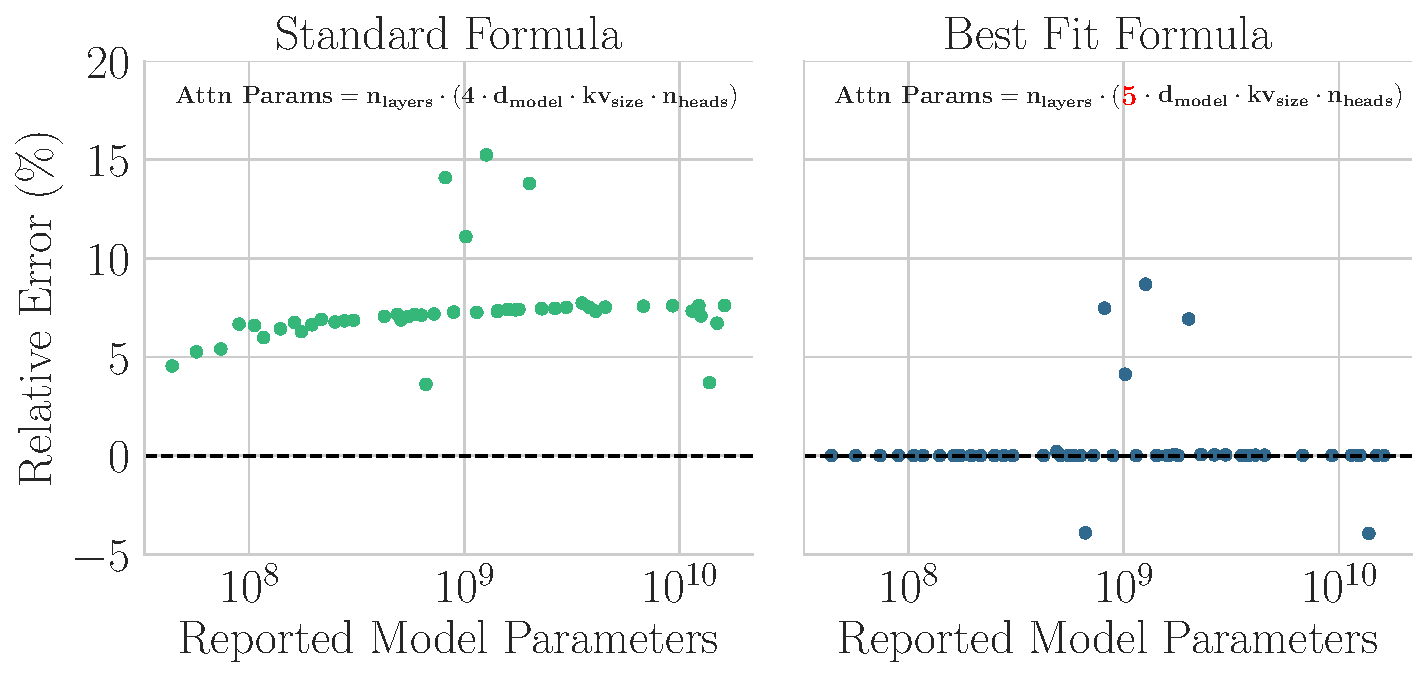
\includegraphics[width=0.85\linewidth]{figures/y=relative_error_x=reported_parameters_hue=equation.pdf}
    \caption{\textbf{Disagreement Between Three Interpretations of Chinchilla's Model Parameters.}
    Each point is one of the 50 models in \citet{hoffman2022chinchilla}'s Table A9.
    \textbf{Left:} Calculating model parameters from the provided architectural hyperparameters using a \textit{standard formula} (Eqn.~\ref{eqn:standard}; attention parameters = $\text{n\_layers} \cdot 4 \cdot \text{d\_model} \cdot \text{kv\_size} \cdot \text{n\_heads}$) disagrees with the reported model parameters for $50/50$ models, with relative errors averaging $7.388\%$ and rising as high as 15.2\%.
    \textbf{Right:} Calculating model parameters using a \textit{best fit formula} (Eqn.~\ref{eqn:bestfit}; replace $4$ with \textcolor{red}{$\mathbf{5}$}) matches $44/50$ of the reported model parameters, and reduces the largest relative error to 8.7\%.
    }
    \label{fig:model_params_bestfit}
\end{figure*}

The field's understanding of scaling models was later altered by the seminal work of \citet{hoffman2022chinchilla}, which introduced the concept of compute-optimal scaling. 
By training over 400 models ranging from 44M to 16B parameters on 5B to 500B tokens, \citet{hoffman2022chinchilla} discovered that producing the best performing model with respect to a fixed pretraining compute budget (``compute-optimal") was achieved by linearly scaling model parameters and pretraining data together.
Chinchilla established the influential ``20-to-1'' heuristic: that the compute-optimal amount of training data is approximately 20 tokens per model parameter (Appendix~\ref{app:theoretical_analysis}).
Their 70B Chinchilla outperformed larger models \citep{rae2022scalinglanguagemodelsmethods}, cementing the methodology as a guiding principle for the field.

However, the precision of this anchor has recently come under scrutiny. Concerns have been raised regarding Chinchilla's wide confidence intervals \citep{zhang2023chinchilla}, internal discrepancies between its analytical approaches \citep{besiroglu2024chinchillascalingreplicationattempt}, and incongruities with other scaling work \citep{porian2024resolvingdiscrepancies, pearce2024reconciling}. As modern training regimes shift toward massive over-training and inference-efficiency, the stability of the Chinchilla baseline is critical; if this foundational coordinate system is unstable, the recipes for modern frontier models become unreliable.
While these works are clear contributions to the science of scaling, the field has been left uncertain: can practitioners still confidently rely on Chinchilla's prescriptions?


In this work, we audit the definitional robustness of the ``Standard Model'' for compute scaling. We begin by uncovering a significant specification error: the model parameters central to the original Chinchilla analyses are ambiguous. As shown in Table~\ref{tab:all_models_abridged} and Figure~\ref{fig:model_params_bestfit}, at least three plausible interpretations of the parameter counts exist:
(1) the model parameters reported in \citet{hoffman2022chinchilla}'s Table A9, (2) the model parameters calculated from the reported model architectural hyperparameters (layers, dimensions, number of heads, etc.) using a ``standard'' formula, and (3) the model parameters calculated from a ``best-fit'' formula.
Although the relative error among these three sets of model parameters rises as high as 15.2\%, we show that key Chinchilla results -- the estimated scaling law parameters and the compute-optimal tokens-per-parameter ratio -- do not meaningfully change. 
In fact, the only potential consequence is that the compute-optimal tokens-per-parameter ratio becomes \textit{more} constant with respect to the target compute budget, strengthening Chinchilla's finding. 

To more generally assess the robustness of compute-optimal scaling, we then study how distorted the model parameters \textit{could} have been without changing Chinchilla's key results.
We perform a sensitivity analysis by perturbing model parameters in four structured ways. 
Our analyses reveals that the robustness depends on the nature of the perturbations: while multiplicative perturbations and random noise have limited effects, additive constants or systematic biases can qualitatively change the compute-optimal scaling strategy by altering the trend of the optimal tokens-to-parameter ratio.
However, overall, all four sensitivity analyses demonstrate that Chinchilla's key results withstand sizable perturbations.
Our results reveal a clear picture: Chinchilla’s compute-optimal prescription remains robust, further justifying its use as a practical scaling blueprint for practitioners.

\noindent\paragraph{Scope:} We do not test whether Chinchilla's functional form extrapolates to modern training regimes; our claims are conditional on the Chinchilla dataset and fitting methods.

% \bmg{I think it's a stronger more clear paper to follow with a final contributions list at the end of the intro. It also sanity checks our paper is novel enough by forcing us to write it. Let me provide a draft and receive feedback, feel free to keep or remove/edit.}
% In summary, our \textbf{main contributions} are:
% \begin{itemize}
%     \item \textit{Identifying Parameter-count ambiguity\footnote{Here, "ambiguity" refers to the fact that the architectural hyperparameters in Hoffmann et al. (2022) lead to multiple internally consistent parameter-count calculations (which we formalize as "standard-formula" and "best-fit" interpretations), neither of which consistently match the parameter counts explicitly reported in the same paper.} in Chinchilla Laws.} We identify a significant ambiguity in Chinchilla’s reported parameter counts, where standard architecture-derived calculations reveal discrepancies as high as 15.2\%.

%     \item \textit{Robustness framework for testing scaling laws.} We propose a general framework for stress-testing the robustness of neural scaling laws by systematically applying four structured perturbations: multiplicative constants, additive constants, systematic biases, and log-normal noise. These perturbations are chosen to model common sources of systematic error in parameter counting (e.g., percentage-based miscalculations or the exclusion of embedding blocks) and to simulate the effects of random, non-systematic factors in training.

%     \item \textit{Power law origin of robustness.} We demonstrate that the observed robustness is an intrinsic property of the power-law form: core scaling exponents are resilient to multiplicative errors that are absorbed into prefactors but are sensitive to additive or systematic errors that structurally break the functional form (e.g., by altering the exponent).
    
%     \item \textit{Tokens-per-parameter constancy.} We show that correcting the identified parameter ambiguity reinforces the Chinchilla “\textasciitilde20-to-1” tokens-to-parameter rule, reducing the ratio’s scaling exponent with compute ($r$ in $\rho_{opt} \propto C^r$) to be even closer to zero.

% \end{itemize}

% The implications of our work are twofold: we provide practitioners with renewed confidence in applying compute-optimal scaling principles, while simultaneously equipping the research community with a framework to rigorously scrutinize and strengthen the foundational scaling laws that guide future AI development.